In the preceding chapter we have seen that the granular temperature could be estimated based on the vector
\begin{equation*}
    \textbf{u}^\text{nst}_p (\textbf{x},\textbf{r},t,a)
    = 
    \frac{1}{P_{nst}(\textbf{x},\textbf{r},t,a)}
    \int \sum_{i}^{N_b}\delta(\textbf{x}-\textbf{x}_i)
    \sum_{j\neq i}^{N_b}\delta(\textbf{x}+\textbf{r}-\textbf{x}_j) 
    \delta(t+a-t_c^{ij}) 
    \textbf{u}_{ij}
    h_{ij} 
    d\mathscr{P}.
    \label{eq:q_nstij}
\end{equation*}
the aim of this chapter is therefore to determine the form of $\textbf{u}^\text{nst}_p$. 

In addition to provides physical explanation the field $\textbf{u}_p^d = \textbf{u}^r_p - \textbf{u}_p$ is of great importance to study the particle phase fluctuation tensor $\avg{\delta_i \textbf{u}_i' \textbf{u}_i'}$ which is of crucial importance in multiphase flow modeling. 
Indeed, it can be shown that 
\begin{equation*}
    \frac{\avg{\delta_i \textbf{u}_i' \textbf{u}_i'}}{n_p}(\textbf{x},t)
    =  
    \int_{\mathbb{R}^3 }
    \textbf{u}_p^d
    \textbf{u}_p^d
    P_{nst}(\textbf{r}|\textbf{x},t)
    d\textbf{r}
    + \int_{\mathbb{R}^3 }
    \textbf{F}(\textbf{r},\textbf{x},t)
    d\textbf{r}
\end{equation*}
where, $\textbf{F} = \avg{\sum_i\sum_{j\neq i}\delta_j\delta_i h_{ij}(\textbf{u}_i - \textbf{u}_p^{nst})(\textbf{u}_i - \textbf{u}_p^{nst})}$. 
Thus, the ensemble averaged particle phase Reynolds stress is the sum of the fluctuation given by $\textbf{u}_p^r$ plus an additional contribution form the others particles fluctuation around the average field $\textbf{u}_p^d$. 


\section{A transport equation for the nearest particle velocity-included pdf properties}

We propose an alternative derivation, to what it is done in \citet{zhang2023evolution} for the derivation of the nearest particle averaged properties. 



The derivation is done by noticing that at the local level we have, 
\begin{align*}
    \pddt \delta(\textbf{x}_i(\FF,t) - \textbf{x})
    + \textbf{u}_i(\FF,t) \cdot \pddx \delta(\textbf{x}_i(\FF,t) - \textbf{x})
    = 0\\
    \pddt \delta(\textbf{u}_i(\FF,t) - \textbf{u})
    + \textbf{a}_i(\FF,t) \cdot \pddu \delta(\textbf{u}_i(\FF,t) - \textbf{u})
    = 0\\
    \pddt \delta(\textbf{x}_j(\FF,t) - \textbf{x}+\textbf{r})
    + \textbf{w}_{ji}(\FF,t) \cdot \pddr \delta(\textbf{x}_j(\FF,t) - \textbf{x}+\textbf{r})
    + \textbf{u}_{i}(\FF,t) \cdot \pddr \delta(\textbf{x}_j(\FF,t) - \textbf{x}+\textbf{r})
    = 0\\
    \pddt \delta(t+a - t^{ij}_c(\FF))
    - \pdda \delta(t+a - t^{ij}_c(\FF))
    = 0,
\end{align*}
where we have defined $\textbf{w}_{ji} = \textbf{u}_j - \textbf{u}_i$ as the relative velocity between particle $j$ and $i$, and $\pddt \textbf{u}_i = \textbf{a}_i$ as the acceleration of the particle . 
For clearly, we note what we call here the \textit{state} function $\Pi$ as, 
\begin{equation*}
    \Pi(\textbf{x},\textbf{r},\textbf{u},t,a,\FF)
    = 
    \sum_i 
    \delta(\textbf{x}_i(\FF,t) - \textbf{x})
    \delta(\textbf{u}_i(\FF,t) - \textbf{u})
    \sum_{j\neq i}\delta(\textbf{x}_j(\FF,t) - \textbf{x}+\textbf{r})
    \delta(t+a - t^{ij}_c(\FF))
    h_{ij}(t,\FF)
\end{equation*}
Then, one may directly deduce that, $\Pi$ follows the conservation equation, 
\begin{equation}
    \pddt \Pi 
    + \pdda \Pi 
    + \pddx\cdot(\textbf{u}_i \Pi)
    + \pddu\cdot(\textbf{a}_{i} \Pi)
    + \pddr\cdot(\textbf{w}_{ji} \Pi)
    = 
    \Pi_S
    \label{eq:dt_Pi}
\end{equation}
where the source term is explicitly defined by, 
\begin{align*}
    \Pi_S
    &= 
    \sum_i 
    \delta(\textbf{x}_i(\FF,t) - \textbf{x})
    \delta(\textbf{u}_i(\FF,t) - \textbf{u})
    \sum_{j\neq i}\delta(\textbf{x}_j(\FF,t) - \textbf{x}-\textbf{r})\\
    &\delta(t+a - t^{ij}_c(\FF))
    h_{ij}(t,\FF)
    \sum_{l\neq i} 
    \delta(r_{li} - r_{jl})
    (\textbf{n}_{li}\cdot\textbf{u}_{li}
     - \textbf{n}_{ji}\cdot \textbf{u}_{ji})\\
    &= 
    \Pi
    \sum_{l\neq i} 
    \delta(r_{li} - r_{jl})
    (\textbf{n}_{li}\cdot\textbf{u}_{li}
     - \textbf{n}_{ji}\cdot \textbf{u}_{ji})\\
\end{align*}
such that 
\begin{align*}
    \iiint \Pi_S  d\PP dS(\textbf{r}) da =
    \iint [\delta(a)P(\textbf{x},\textbf{r},\textbf{u},t,0)
    - \frac{P_\text{nst}(\textbf{x},\textbf{r},,\textbf{u}t,a)}{\tau^\text{nst}(\textbf{x},\textbf{r},\textbf{u},t,a)}] dS(\textbf{r}) da
    = 0 
\end{align*}
is a source terms related to the inter-changes in nearest neighbors. 

Firstly, note that integrating \ref{eq:dt_Pi} on all configurations yields the same conservation equation as \citet{zhang2023evolution} for $P_\text{nst}$. 
Making our derivation consistent with his. 


To derive an equation for $\textbf{u}_p^\text{nst}$ the process is easy, 
we simply multiply \ref{eq:dt_Pi} by $\textbf{u}_i$ and average on all configurations. 
It yields, 
\begin{equation*}
    \pddt \avg{\Pi \textbf{u}_i}
    + \pdda \avg{\Pi  \textbf{u}_i}
    + \pddx\cdot\avg{\textbf{u}_i \textbf{u}_i  \Pi}
    + \pddu\cdot\avg{\textbf{a}_i \textbf{u}_i  \Pi}
    + \pddr\cdot \avg{ \textbf{u}_i \textbf{w}_{ji} \Pi}
    = 
    \avg{\Pi_S \textbf{u}_i}
    + \avg{\Pi \textbf{a}_i }
\end{equation*}
Noticing that, $\avg{\textbf{u}_i \Pi} = \textbf{u}P_\text{nst}$ we directly obtain the equation for \textbf{u}:
\begin{multline*}
    \pddt (\textbf{u} P_\text{nst})
    + \pdda (\textbf{u} P_\text{nst})
    + \pddx \cdot  (\textbf{u} \textbf{u}  P_\text{nst})
    + \pddr \cdot  (\textbf{u}\textbf{w}^\text{nst}_p P_\text{nst})
    + \pddu \cdot  (\textbf{u}\textbf{a}^\text{nst}_p P_\text{nst})\\
    = \textbf{u} 
    \left[\delta(a)  P(\textbf{x},\textbf{r}, \textbf{u},t,0)
    - \frac{P_\text{nst}(\textbf{x},\textbf{r},\textbf{u},t,a)}{\tau^\text{nst}(\textbf{x},\textbf{r},\textbf{u},t,a)}
    \right]
    + \textbf{a}_p^\text{nst}
    P_\text{nst} 
\end{multline*}


With our new notation we have shown that we have the exact notation, 
\begin{equation*}
    \avg{\delta_i \textbf{u}_i' \textbf{u}_i'}
    = 
    \int 
    \textbf{uu}
    P_\text{nst}(\textbf{x},\textbf{r},\textbf{u},a,t)
    d\textbf{r}
    d\textbf{u}
    da
    - \textbf{u}_p \textbf{u}_p n_p
\end{equation*}
Thus, we rather derive the previous equation by \textbf{u} which gives, 
\begin{multline*}
    \pddt (\textbf{uu} P_\text{nst})
    + \pdda (\textbf{uu} P_\text{nst})
    + \pddx \cdot  (\textbf{uu} \textbf{u}  P_\text{nst})
    + \pddr \cdot  (\textbf{uu}\textbf{w}^\text{nst}_p P_\text{nst})
    + \pddu \cdot  (\textbf{uu}\textbf{a}^\text{nst}_p P_\text{nst})\\
    = \textbf{uu} 
    \left[\delta(a)  P(\textbf{x},\textbf{r}, \textbf{u},t,0)
    - \frac{P_\text{nst}(\textbf{x},\textbf{r},\textbf{u},t,a)}{\tau^\text{nst}(\textbf{x},\textbf{r},\textbf{u},t,a)}
    \right]
    + \textbf{u}\textbf{a}_p^\text{nst}
    + \textbf{a}_p^\text{nst}\textbf{u}
    P_\text{nst} 
\end{multline*}
integrating Overall age and velocity and relative position gives, 
\begin{equation*}
    \pddt (n_p \textbf{F}_p )
    +\pddx (n_p\textbf{F}_p \textbf{u}_p  + n_p \textbf{F}^{Re})
    = 
    - \frac{n_p \textbf{F}_p }{\tau_p}
    + n_p \textbf{B}_p
    + n_p \textbf{D}_p
    + n_p \textbf{A}_p
\end{equation*}
with, 
\begin{align*}
    n_p \textbf{F}^{Re}(\textbf{x},t)
    =
    \int_{0}^\infty
    \int_{\mathbb{R}^6}
    \textbf{uu}(\textbf{u}- \textbf{u}_p)
    P(\textbf{x},\textbf{r},t,a)
    d\textbf{r}
    d\textbf{u}
    da,\\
    n_p \textbf{B}(\textbf{x},t)
    =
    \int_{0}^\infty
    \int_{\mathbb{R}^6}
    \textbf{uu}
    P(\textbf{x},\textbf{r},t,0)\delta(a)
    d\textbf{r}
    d\textbf{u}
    da, \\
    n_p\textbf{D}(\textbf{x},t) = 
    \int_{0}^\infty
    \int_{\mathbb{R}^6} \textbf{uu}
    \left[
        \frac{1}{\tau_p(\textbf{x},t)}
        - \frac{1}{\tau^\text{nst}(\textbf{x},\textbf{r},t,a)}
    \right]
    P_\text{nst}
    d\textbf{r}
    d\textbf{u}
    da,\\
    n_p \textbf{W}(\textbf{x},t) = 
    \int_{0}^\infty
    \int_{\mathbb{R}^6} \left[
        \textbf{u} \textbf{a}^\text{nst}_p
        + \textbf{a}^\text{nst}_p\textbf{u}
    \right]P_\text{nst}
    d\textbf{r}
    d\textbf{u}
    da.
\end{align*} 
Which is a global evolution equation for the particle tensor. 
However, note how this is pointless since one may directly note that, 
\begin{align*}
    \int\iiint \textbf{uu}\Pi_S  d\PP dS(\textbf{r}) da d\textbf{u} dr =
    \iint \textbf{uu} 
    \iint [\delta(a)P(\textbf{x},\textbf{r},\textbf{u},t,0)
    - \frac{P_\text{nst}(\textbf{x},\textbf{r},,\textbf{u}t,a)}{\tau^\text{nst}(\textbf{x},\textbf{r},\textbf{u},t,a)}] dS(\textbf{r}) da
    dr d \textbf{u}
    = 0 
\end{align*}
Indeed, since $\textbf{u}$ is not explicitly related to the particle relative position, this is not affected by this source term.. . 
And therefore, 
\begin{equation*}
    \pddt (n_p \textbf{F}_p )
    +\pddx (n_p\textbf{F}_p \textbf{u}_p  + n_p \textbf{F}^{Re})
    = 
    \int_{0}^\infty
    \int_{\mathbb{R}^6} \left[
        \textbf{u} \textbf{a}^\text{nst}_p
        + \textbf{a}^\text{nst}_p\textbf{u}
    \right]P_\text{nst}
    d\textbf{r}
    d\textbf{u}
    da.
\end{equation*}

\begin{figure}[h!]
    \centering
    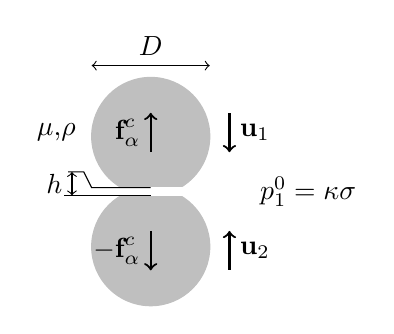
\begin{tikzpicture}
      \draw[lightgray,fill = lightgray] (0,0.7) circle (0.75);
      \draw[lightgray,fill = lightgray] (0,-0.7) circle (0.75);
      \draw[white,fill=white] (-0.75,-0.05) rectangle (0.75,0.05);
      \draw(0,0.05)--++(-0.75,0)--++(-0.1,0.2)--++(-0.2,0);
      \draw(0,-0.05)--++(-1.1,0);
      \draw[<->](-1,-0.05) --++ (0,0.3)node[midway,left]{$h$};
      \draw[<->](-0.75,1.6)--++(1.5,0)node[midway,above]{$D$};
      \node (para) at (-1.2,0.75){$\mu$,$\rho$};
      \node (pressure) at (2,0){$p_1^0 = \kappa \sigma$};
      \draw[->,thick](0,0.5)--++(0,0.5)node[midway,left]{$\textbf{f}_\alpha^\text{c}$};
      \draw[->,thick](0,-0.5)--++(0,-0.5)node[midway,left]{$-\textbf{f}_\alpha^\text{c}$};
      \draw[<-,thick](1,0.5)--++(0,0.5)node[midway,right]{$\textbf{u}_1$};
      \draw[<-,thick](1,-0.5)--++(0,-0.5)node[midway,right]{$\textbf{u}_2$};
    \end{tikzpicture}
    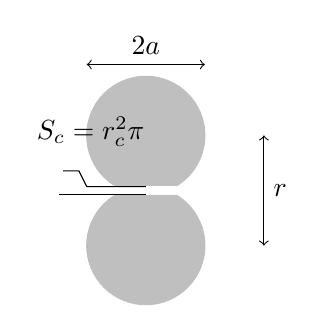
\begin{tikzpicture}
      \draw[lightgray,fill = lightgray] (0,0.7) circle (0.75);
      \draw[lightgray,fill = lightgray] (0,-0.7) circle (0.75);
      \draw[white,fill=white] (-0.75,-0.05) rectangle (0.75,0.05);
      \draw(0,0.05)--++(-0.75,0)--++(-0.1,0.2)--++(-0.2,0);
      \draw(0,-0.05)--++(-1.1,0);
      \draw[<->](-0.75,1.6)--++(1.5,0)node[midway,above]{$2 a$};
      \draw[<->](1.5,0.7)--++(0,-1.4)node[midway,right]{$r$};
      \node (para) at (-0.7,0.75){$S_c = r_c^2 \pi$};
    \end{tikzpicture}
    \caption{Scheme of two colliding droplets at close contact. Note the null kurvature in the region of the interface close to the film leading to a capilary force $\textbf{f}_\alpha^\text{c} \approx - S_c \kappa \sigma \textbf{r}/|\textbf{r}|$. }
\end{figure}
the inter particle force 
\begin{equation*}
    \textbf{f}_{ij}^\text{c}
    = S_c \kappa \gamma \textbf{r}_{ij}/r_{ij}
    = \pi r_c^2 \kappa \gamma \textbf{r}_{ij}/r_{ij}
    = \pi (a^2 - r_{ij}^2/4) \kappa \gamma  \textbf{r}_{ij}/r_{ij}
\end{equation*} 
where the 
The resultants of these forces on the particle $i$ is therefore the sum of the contact with all particles except the $j^\text{th}$ particle, 
\begin{equation*}
    \textbf{f}_{i}^\text{c}
    = \sum_{j \neq i}\textbf{f}_{ij}
    = - \sum_{j \neq i} \pi (a^2 - r_{ij}^2/4) \kappa \gamma \textbf{r}_{ij}/r_{ij}
\end{equation*} 
The relative acceleration might be written as, 
\begin{equation*}
    a_p^\text{nst}
    = 
    \pi (a^2 - r^2/4) \kappa \gamma \textbf{r}/r
\end{equation*}
where we assume that the force is only due to the only nearest neighbor. 
Thus, 
\begin{equation*}
    \int_{0}^\infty
    \int_{\mathbb{R}^6} \left[
        \textbf{u} \textbf{a}^\text{nst}_p
    \right]P_\text{nst}
    d\textbf{r}
    d\textbf{u}
    da.
    = 
    \int_{0}^\infty
    \int_{\mathbb{R}^6} \left[
        \textbf{u} \pi (a^2/r - r/4) \kappa \gamma \textbf{r}
    \right]P_\text{nst}
    d\textbf{r}
    d\textbf{u}
    da
\end{equation*}


\subsection{Let remove the condition on $\textbf{u}_i$ for $\Pi$. }
It gives, 
\begin{equation*}
    \avg{\delta_i \textbf{u}_i' \textbf{u}_i'}(\textbf{x},t)
    =  
    \int_{\mathbb{R}^3 }
    (\textbf{u}_p^\text{nst} -\textbf{u}_p)
    (\textbf{u}_p^\text{nst} - \textbf{u}_p)
    P_{nst}(\textbf{r},\textbf{x},a,t)
    d\textbf{r}
    + \int_{\mathbb{R}^3 }
    \textbf{F}(\textbf{r},\textbf{x},t)
    d\textbf{r}
\end{equation*}
where, $\textbf{F} = \avg{\Pi (\textbf{u}_i - \textbf{u}_p^{nst})(\textbf{u}_i - \textbf{u}_p^{nst})}$. 

\begin{equation*}
    \pddt \avg{\Pi \textbf{u}_i}
    + \pdda \avg{\Pi  \textbf{u}_i}
    + \pddx\cdot\avg{\textbf{u}_i \textbf{u}_i  \Pi}
    + \pddr\cdot \avg{ \textbf{u}_i \textbf{w}_{ji} \Pi}
    = 
    \avg{\Pi_S \textbf{u}_i}
    + \avg{\Pi \textbf{a}_i }
\end{equation*}
which gives, 
\begin{multline*}
    \pddt (\textbf{u}_p^\text{nst} P_\text{nst})
    + \pdda (\textbf{u}_p^\text{nst} P_\text{nst})
    + \pddx \cdot  (\textbf{u}_p^\text{nst} \textbf{u}^\text{nst}  P_\text{nst} + \textbf{u}^{Re})
    + \pddr \cdot  (\textbf{u}_p^\text{nst} \textbf{w}^\text{nst}_p P_\text{nst}+ \textbf{w}^{Re})\\
    = \delta(a)  \textbf{u}_p^\text{nst} P(\textbf{x},\textbf{r}, \textbf{u},t,0)
    - \frac{ \textbf{u}_p^{nst}(|D) P_\text{nst}(\textbf{x},\textbf{r},\textbf{u},t,a)}{\tau^\text{nst}(\textbf{x},\textbf{r},\textbf{u},t,a)}
    + \textbf{a}_p^\text{nst}
    P_\text{nst} 
\end{multline*}

\subsection*{Model for the conditioned acceleration based on numerical results}